% !TEX root = ieee_gossip_comparison_report.tex
\documentclass[conference]{IEEEtran}

\usepackage{amsmath}
\usepackage{amssymb}
\usepackage{array}
\usepackage{graphicx}
\usepackage{url}
\graphicspath{{./}{reports/}{plots_epsilon_lambda/}}

\title{Simulation Study of Randomized Gossip, Geographic Gossip, and Randomized Path Averaging}

\author{
\IEEEauthorblockN{Gossip Framework Simulation Report}
\IEEEauthorblockA{Generated from 100-node, 50-trial topology benchmarks}
}

\begin{document}
\maketitle

\begin{abstract}
Distributed averaging is a canonical consensus problem for sensor, ad hoc, and peer-to-peer networks. Classical randomized gossip is simple and robust, but on geometric and grid-like networks it mixes slowly because information diffuses only through local neighbor exchanges. Geographic gossip accelerates convergence by routing to distant nodes using location information, while randomized path averaging further exploits the routed path by averaging every node visited by the packet. This report compares these three algorithms in a common simulation framework across five network topologies: complete, Erdos-Renyi random, random geometric, ring, and scale-free graphs. The experiments use 100 nodes, 50 independent topology instances per topology, and an absolute consensus threshold of $10^{-2}$. The results support the main message of the literature: long-range geographic communication reduces averaging time, and averaging along paths is especially effective on sparse geometric or grid-like networks. On the ring topology, nearest-neighbor randomized averaging did not converge within 20,000 rounds in any run, while path averaging converged in 25.3 rounds on average using 1,263 one-hop transmissions. On random geometric graphs, path averaging was the fastest algorithm and, among converged runs, used fewer messages than both the standard and geographic methods.
\end{abstract}

\section{Problem Definition}
Let $G=(V,E)$ be a connected communication graph with $|V|=n$. Each node $i \in V$ starts with a scalar measurement $x_i(0)$. The distributed averaging problem is to drive all node estimates to
\begin{equation}
    \bar{x} = \frac{1}{n}\sum_{i=1}^{n}x_i(0),
\end{equation}
using only message passing over graph edges. Let $x(t) \in \mathbb{R}^{n}$ denote the vector of estimates after round $t$. A valid averaging protocol preserves the global sum and has $\bar{x}\mathbf{1}$ as a fixed point:
\begin{equation}
    \mathbf{1}^{T}W(t)=\mathbf{1}^{T}, \qquad W(t)\mathbf{1}=\mathbf{1},
\end{equation}
where $x(t+1)=W(t)x(t)$ is the random update induced by the algorithm.

Following Boyd et al.~\cite{boyd2006randomized} and the geographic/path averaging papers~\cite{dimakis2006geographic,benezit2008order}, convergence can be described by an $\epsilon$-averaging time:
\begin{equation}
T_{\mathrm{ave}}(\epsilon)
= \sup_{x(0)}
\inf\left\{t:
\Pr\left(
\frac{\|x(t)-\bar{x}\mathbf{1}\|}{\|x(0)\|}\geq \epsilon
\right)\leq \epsilon
\right\}.
\end{equation}
For i.i.d. symmetric averaging matrices, the rate is governed by the second largest eigenvalue in magnitude of the expected update matrix:
\begin{equation}
T_{\mathrm{ave}}(\epsilon)
= \Theta\left(
\frac{\log \epsilon^{-1}}{1-\lambda_2(\mathbb{E}[W])}
\right).
\label{eq:spectral}
\end{equation}
The simulations in this report use an empirical stopping rule: a run is marked converged when
\begin{equation}
    \max_i |x_i(t)-\bar{x}| < 10^{-2}.
\end{equation}

The main cost metric is the number of one-hop transmissions. If $R(t)$ is the number of one-hop transmissions in round $t$, then the expected communication cost is
\begin{equation}
    C_{\mathrm{ave}}(\epsilon)=\mathbb{E}[R(1)]T_{\mathrm{ave}}(\epsilon),
\end{equation}
and the empirical cost used in the benchmark is
\begin{equation}
    \widehat{C}=\sum_{t=0}^{\widehat{T}-1}R(t),
\end{equation}
where $\widehat{T}$ is the observed number of simulator rounds.

\section{Algorithms}
\subsection{Randomized Nearest-Neighbor Averaging}
The baseline algorithm is standard randomized pairwise gossip. At each asynchronous clock tick, one active node $i$ is selected uniformly and chooses a neighbor $j$ according to a transition rule. In our simulation, the transition is uniform over the neighbors of $i$. The pair replaces both estimates with their average:
\begin{equation}
    x_i(t+1)=x_j(t+1)=\frac{x_i(t)+x_j(t)}{2}.
\end{equation}
Equivalently, the update matrix is
\begin{equation}
    W_{ij}=I-\frac{1}{2}(e_i-e_j)(e_i-e_j)^T.
\end{equation}
This protocol is fully local and uses one one-hop transmission per clock tick in our accounting. Its drawback is that information propagates diffusively. On grids and random geometric graphs, the path averaging paper summarizes the expected communication cost as
\begin{equation}
    C_{\mathrm{ave}}^{\mathrm{std}}
    = \Theta(n^2\log\epsilon^{-1})
\end{equation}
on grids, and
\begin{equation}
    C_{\mathrm{ave}}^{\mathrm{std}}
    = \Theta\left(\frac{n^2\log\epsilon^{-1}}{\log n}\right)
\end{equation}
on random geometric graphs~\cite{benezit2008order}. This slow scaling is what we expect on sparse, local topologies such as the ring and random geometric graph.

\subsection{Geographic Gossip}
Geographic gossip assumes nodes know their own coordinates and the coordinates of neighbors. Rather than average with a one-hop neighbor, a source node samples a target point uniformly in the deployment region and greedily routes toward that point. The reached node is used as a distant gossip partner. The endpoint pair then averages:
\begin{equation}
    x_s(t+1)=x_v(t+1)=\frac{x_s(t)+x_v(t)}{2}.
\end{equation}
In the geographic gossip analysis, random target locations induce a nonuniform distribution over sensors because nodes with larger Voronoi cells are sampled more often. Rejection sampling is used to temper this bias. If $P_{ij}$ is the probability that node $i$ exchanges values with node $j$, then the expected pairwise gossip matrix can be written as
\begin{equation}
    W = I + \frac{1}{2n}(P+P^T-D),
\end{equation}
where $D$ is diagonal with $D_i=\sum_j(P_{ij}+P_{ji})$~\cite{dimakis2006geographic}. The key gain is that greedy routing creates an overlay that behaves more like a complete graph. The paper proves
\begin{equation}
    T_{\mathrm{ave}}^{\mathrm{geo}}(\epsilon)
    = \Theta(n\log\epsilon^{-1})
\end{equation}
for random geometric graphs, while each routed exchange costs about
\begin{equation}
    \mathbb{E}[R] = \Theta\left(\sqrt{\frac{n}{\log n}}\right)
\end{equation}
one-hop transmissions. Thus,
\begin{equation}
    C_{\mathrm{ave}}^{\mathrm{geo}}
    = \Theta\left(
    \frac{n^{3/2}\log\epsilon^{-1}}{\sqrt{\log n}}
    \right).
\end{equation}

\subsection{Randomized Path Averaging}
Randomized path averaging modifies geographic gossip by averaging every node on the routed path, not just the source and destination. If $S(t)$ is the set of nodes on the route, then every node $k\in S(t)$ updates to
\begin{equation}
    x_k(t+1)=\frac{1}{|S(t)|}\sum_{\ell\in S(t)}x_\ell(t),
\end{equation}
while nodes outside the path remain unchanged. The corresponding averaging matrix is a projection:
\begin{equation}
W_{k\ell}(t)=
\begin{cases}
1/|S(t)|, & k,\ell\in S(t),\\
1, & k=\ell,\; k\notin S(t),\\
0, & \text{otherwise.}
\end{cases}
\end{equation}
The intuition is simple but powerful: the multi-hop route has already paid to visit intermediate nodes, so aggregating their values and sending the path average back along the same route costs little extra relative to endpoint-only geographic gossip.

Benezit et al.~\cite{benezit2008order} analyze a box-path variant of this idea using the travel agency method, which applies Markov-chain canonical path bounds to $\lambda_2(\mathbb{E}[W])$. Their main comparison for grids and random geometric graphs is
\begin{equation}
    C_{\mathrm{ave}}^{\mathrm{path}}
    = \Theta(n\log\epsilon^{-1}),
\end{equation}
which is order-optimal up to the logarithmic accuracy factor because at least $\Omega(n)$ messages are required to average $n$ initial measurements.

Our implementation follows the practical random greedy version described in the path averaging paper: a source samples a target point in $[0,1]^2$, repeatedly chooses a random unvisited neighbor that is closer to the target, stops at a local minimum, averages all nodes on the route, and counts $2(|S|-1)$ one-hop transmissions for forward aggregation plus reverse dissemination.

\section{Simulation Setup}
All experiments were run in the local gossip framework. Each run used $n=100$ nodes, independent initial values sampled uniformly from $[0,1]$, and a convergence threshold of $10^{-2}$. For each topology, 50 independent topology instances were generated. Each algorithm was run once per instance using the same initial values and topology seed for fairness. The maximum number of rounds was 20,000.

\subsection{Network Topologies}
Figure~\ref{fig:topology_examples} shows small illustrative examples of the five topology families used in the benchmark.

\begin{figure*}[t]
\centering
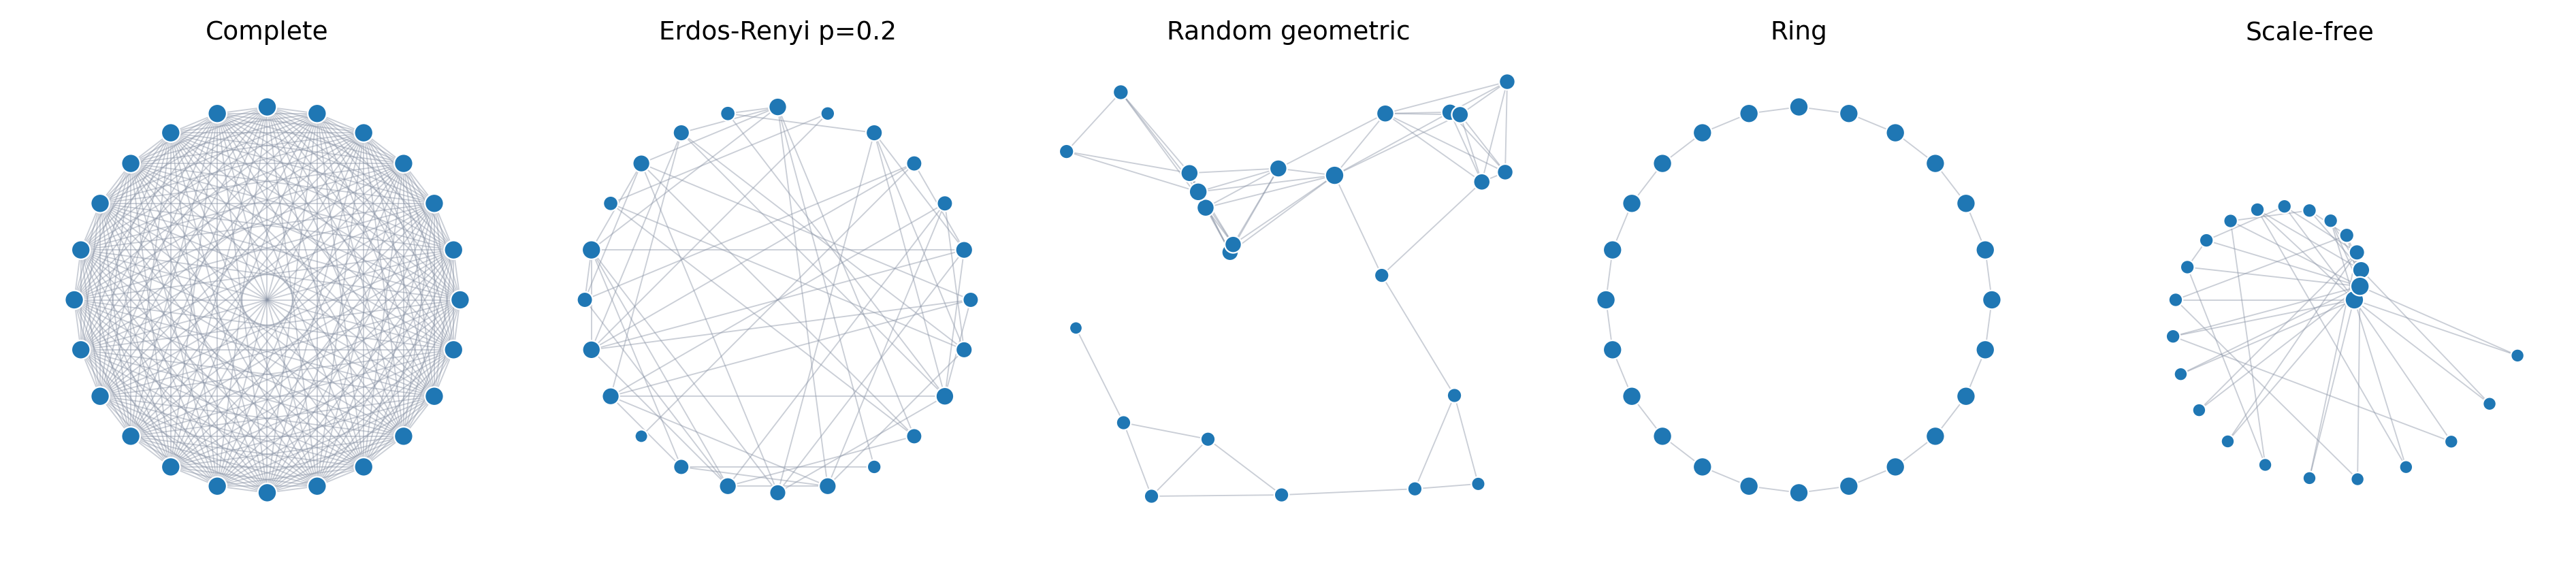
\includegraphics[width=\textwidth]{topology_examples.png}
\caption{Example 24-node visualizations of the topology families used in the experiments. The benchmark itself uses 100-node instances.}
\label{fig:topology_examples}
\end{figure*}

\textbf{Complete graph.}
In the complete graph, every pair of nodes is connected by a direct communication edge. This is the densest topology in the study and acts as a high-connectivity reference case: information can move globally after a single neighbor selection, so the ordinary nearest-neighbor baseline is already strong. Geographic and path averaging can reduce the number of rounds, but their routed exchanges do not exploit a locality bottleneck because there is almost no bottleneck to remove.

\textbf{Erdos-Renyi random graph.}
In the Erdos-Renyi topology, each possible edge is included independently with probability $p=0.2$. This produces a graph that is much sparser than the complete graph but still has many shortcut edges. It is useful as an intermediate random network: unlike the ring or random geometric graph, communication is not constrained to local neighborhoods, so long-range mixing is often available even without geographic routing.

\textbf{Random geometric graph.}
In the random geometric topology, nodes are placed uniformly in $[0,1]^2$ and two nodes are connected when their Euclidean distance is at most $r=\sqrt{\log(n)/n}$. This is the topology most closely aligned with wireless sensor-network models, where edges represent local radio range. It is also the topology where geographic gossip and path averaging are expected to help most, because long-range information movement requires routed multi-hop paths through local edges.

\textbf{Ring.}
In the ring topology, nodes are arranged on a cycle and each node has exactly two neighbors. It is the sparsest connected topology in the benchmark and has a very small spectral gap, so ordinary pairwise averaging spreads information slowly around the cycle. The ring is therefore a stress test for locality: endpoint-only geographic gossip pays for long routes, while path averaging turns those same routes into useful multi-node averaging operations.

\textbf{Scale-free graph.}
The scale-free topology is generated using a Barabasi-Albert-style preferential attachment rule with $m=2$. A few high-degree hub nodes receive many edges, while most nodes have low degree. This creates natural shortcuts through hubs, so the graph is sparse but not purely local. As a result, path averaging still helps reduce rounds, but the advantage is smaller than on the ring or random geometric graph because hub structure already supports long-range mixing.

The algorithms compared were:
\begin{itemize}
    \item \texttt{base\_random\_avg}: nearest-neighbor randomized averaging with one clock tick per simulator round.
    \item \texttt{geographic}: greedy geographic endpoint averaging with Voronoi rejection sampling.
    \item \texttt{path\_avg}: randomized greedy path averaging.
\end{itemize}
The output file for the benchmark is \url{results/base_geo_path_all_topologies_benchmark_100nodes_50runs.csv}.

\subsection{Spectral Bound Check for Random Averaging}
As a correctness check for the nearest-neighbor randomized averaging implementation, we separately compared empirical convergence times against the spectral estimate used in the randomized gossip literature. For a fixed topology and its expected one-clock-tick update matrix, the plotting script computes
\begin{equation}
    \widehat{T}(\epsilon)
    =
    \frac{\log(1/\epsilon)}{\log(1/\lambda_2)},
    \label{eq:lambda_runtime_estimate}
\end{equation}
where $\lambda_2$ is the second-largest eigenvalue in magnitude of $\mathbb{E}[W]$. The shaded region in Figure~\ref{fig:epsilon_lambda_plots} uses constant-factor lower and upper curves
\begin{equation}
    T_{\mathrm{lower}}(\epsilon)
    =
    \frac{1}{2}
    \frac{\log(1/\epsilon)}{\log(1/\lambda_2)},
    \qquad
    T_{\mathrm{upper}}(\epsilon)
    =
    3
    \frac{\log(1/\epsilon)}{\log(1/\lambda_2)}.
    \label{eq:lambda_bounds}
\end{equation}
These are not fitted to the data; they are constant-factor envelopes around the standard spectral convergence expression.

The validation run used $n=100$, the random averaging algorithm, $\epsilon\in\{10^{-1},5\times10^{-2},10^{-2},5\times10^{-3},10^{-3}\}$, and a maximum of 300,000 rounds per trial. The ring topology is the important stress case: with $\lambda_2$ very close to one, the stricter thresholds required 101,517 rounds at $\epsilon=10^{-2}$ and 217,807 rounds at $\epsilon=10^{-3}$. This explains why the shorter 20,000-round benchmark cap was too small for baseline random averaging on the ring.

For looser thresholds the ring can appear faster than the lower curve suggests. This does not indicate a bug in the averaging update. The theoretical $T_{\mathrm{ave}}(\epsilon)$ is a worst-case, probability-based quantity, while the plotted experiment is a single empirical trajectory from a random initial state and stops when the maximum absolute error falls below the chosen threshold. Random initial states may have a small projection on the ring's slowest Fourier modes, so early coarse-error reduction can be much faster than the worst-case spectral envelope. As $\epsilon$ is tightened, the slow modes dominate and the observed ring runtime moves into the same order as the spectral prediction.

\begin{figure*}[t]
\centering
\begin{minipage}{0.49\textwidth}
\centering

\includegraphics[width=\textwidth]{theory_vs_empirical_Complete.png}
\end{minipage}
\hfill
\begin{minipage}{0.49\textwidth}
\centering

\includegraphics[width=\textwidth]{theory_vs_empirical_Random_p=0.2.png}
\end{minipage}

\vspace{0.5em}
\begin{minipage}{0.49\textwidth}
\centering

\includegraphics[width=\textwidth]{theory_vs_empirical_Ring.png}
\end{minipage}
\hfill
\begin{minipage}{0.49\textwidth}
\centering

\includegraphics[width=\textwidth]{theory_vs_empirical_Scale-free.png}
\end{minipage}
\caption{Spectral bound check for randomized nearest-neighbor averaging on four topology families. The shaded bands use Equations~\eqref{eq:lambda_runtime_estimate} and~\eqref{eq:lambda_bounds}; empirical points are simulator stopping times for the same fixed topology instance.}
\label{fig:epsilon_lambda_plots}
\end{figure*}

\section{Results}
Table~\ref{tab:results} summarizes the 750 simulation runs. The reported means and standard deviations include capped runs that did not reach the threshold by 20,000 rounds.

\begin{table*}[t]
\centering
\caption{Benchmark results for 100 nodes, 50 instances per topology, threshold $10^{-2}$.}
\label{tab:results}
\begin{tabular}{llcccl}
\hline
Topology & Algorithm & Converged & Rounds & Messages & Final error \\
\hline
complete & base\_random\_avg & 50/50 & 945.3 $\pm$ 117.4 & 945.3 $\pm$ 117.4 & 0.007915 \\
complete & geographic & 50/50 & 969.8 $\pm$ 94.4 & 2199.8 $\pm$ 219.3 & 0.00806 \\
complete & path\_avg & 50/50 & 243.3 $\pm$ 42.7 & 2046.5 $\pm$ 366.3 & 0.006434 \\
random\_p02 & base\_random\_avg & 50/50 & 987.7 $\pm$ 96.7 & 987.7 $\pm$ 96.7 & 0.007788 \\
random\_p02 & geographic & 50/50 & 1052.6 $\pm$ 143.8 & 3161.7 $\pm$ 457.0 & 0.00761 \\
random\_p02 & path\_avg & 50/50 & 379.7 $\pm$ 66.4 & 2262.9 $\pm$ 374.0 & 0.006936 \\
random\_geometric & base\_random\_avg & 48/50 & 5562.2 $\pm$ 3499.2 & 5562.2 $\pm$ 3499.2 & 0.01665 \\
random\_geometric & geographic & 48/50 & 1785.7 $\pm$ 3758.3 & 13434.5 $\pm$ 27201.8 & 0.01502 \\
random\_geometric & path\_avg & 48/50 & 1014.2 $\pm$ 3915.1 & 12158.4 $\pm$ 46606.7 & 0.01315 \\
ring & base\_random\_avg & 0/50 & 20000.0 $\pm$ 0.0 & 20000.0 $\pm$ 0.0 & 0.04373 \\
ring & geographic & 50/50 & 923.3 $\pm$ 99.7 & 48646.2 $\pm$ 5423.5 & 0.008281 \\
ring & path\_avg & 50/50 & 25.3 $\pm$ 10.6 & 1263.0 $\pm$ 455.4 & 0.006415 \\
scale\_free & base\_random\_avg & 50/50 & 2028.9 $\pm$ 246.5 & 2028.9 $\pm$ 246.5 & 0.00894 \\
scale\_free & geographic & 50/50 & 2010.7 $\pm$ 274.9 & 4644.4 $\pm$ 638.5 & 0.008425 \\
scale\_free & path\_avg & 50/50 & 1169.5 $\pm$ 222.4 & 3481.0 $\pm$ 652.7 & 0.007428 \\
\hline
\end{tabular}
\end{table*}

\subsection{Sparse Local Topologies}
The ring graph is the clearest confirmation of the theory. The ring is not a random geometric graph, but it is a sparse local topology with poor spectral gap. The baseline method never reached the threshold within 20,000 rounds. Geographic gossip converged in 923.3 rounds on average, but paid 48,646 one-hop transmissions because each endpoint exchange required long routing around the cycle. Path averaging converged in only 25.3 rounds and 1,263 messages. This result directly reflects the paper's argument: if a message must traverse a long route, averaging all nodes on that route uses the communication far more efficiently than averaging only the endpoints.

\subsection{Random Geometric Graphs}
The random geometric graph is the topology most directly connected to the geographic and path averaging papers. All three algorithms failed on the same two topology instances, which suggests a graph/topology limitation rather than an algorithm-specific failure. This is plausible because the simulation radius $r=\sqrt{\log n/n}$ is less conservative than the larger constants used in theoretical high-probability connectivity arguments. Among the 48 converged random geometric instances, the average costs were:
\begin{equation}
\begin{aligned}
\widehat{C}_{\mathrm{std}} &\approx 4960.6,\\
\widehat{C}_{\mathrm{geo}} &\approx 7942.3,\\
\widehat{C}_{\mathrm{path}} &\approx 2741.8.
\end{aligned}
\end{equation}
Thus, path averaging used about 55\% of the standard gossip messages and about 35\% of the geographic gossip messages on converged random geometric runs, while also requiring far fewer rounds. This is the strongest match to the asymptotic comparison $C_{\mathrm{ave}}^{\mathrm{std}} > C_{\mathrm{ave}}^{\mathrm{geo}} > C_{\mathrm{ave}}^{\mathrm{path}}$ for geometric networks.

\subsection{Dense and Hub-Dominated Topologies}
On complete and Erdos-Renyi graphs, path averaging reduced rounds but not always total messages relative to the nearest-neighbor baseline. For example, on the complete graph path averaging reached the threshold in 243.3 rounds, about one quarter of the baseline rounds, but used 2,046.5 messages because each round averaged a multi-hop greedy path. This is not a contradiction of the papers: geographic and path averaging are designed to overcome locality bottlenecks in sparse geometric networks. In dense networks, a one-hop randomized exchange is already effective, so the extra path cost can dominate.

The scale-free topology shows an intermediate behavior. The path algorithm reduced rounds from 2,028.9 to 1,169.5 and used fewer messages than geographic gossip, but still used more messages than baseline randomized averaging. This reflects the presence of hubs: long-range mixing already exists structurally, so routed path averaging helps less than it does on the ring or random geometric graph.

\subsection{Spectral Interpretation}
Equation~\eqref{eq:spectral} predicts slow convergence when $1-\lambda_2(\mathbb{E}[W])$ is small. The empirical topology gaps computed for the baseline expected gossip matrix follow the observed difficulty: the complete graph had average spectral gap about $1.01\times 10^{-2}$ and converged quickly, while the ring had gap about $2.0\times 10^{-5}$ and did not converge under baseline gossip. Geographic and path averaging effectively change the update matrix by creating long-range averaging events, increasing the practical information flow even though the physical graph remains sparse.

\section{Conclusion}
The simulations reproduce the qualitative hierarchy established in the three papers. Standard randomized averaging is robust and simple, but it is bottlenecked by the physical graph's local mixing properties. Geographic gossip uses location information to create long-range endpoint exchanges and greatly reduces the number of rounds on sparse local networks, although the routed messages can be expensive. Randomized path averaging obtains the best overall behavior on the topologies where the theory predicts it should: sparse local graphs where messages must traverse many intermediate nodes. The ring and random geometric results are especially aligned with the order-optimal path averaging argument, because averaging the entire route converts routing overhead into useful consensus work.

The main caveat is that the experiment uses finite graphs with $n=100$ and a practical greedy-routing implementation. The random geometric graph radius also produced two hard instances where no algorithm reached threshold by the 20,000-round cap. A natural next step is to run a scaling study over larger $n$ and multiple geometric radius constants $r(n)=\sqrt{c\log n/n}$, which would make the asymptotic claims in the papers visible as slopes in message complexity.

\begin{thebibliography}{1}

\bibitem{boyd2006randomized}
S. Boyd, A. Ghosh, B. Prabhakar, and D. Shah, ``Randomized gossip algorithms,'' \emph{IEEE Transactions on Information Theory}, vol. 52, no. 6, pp. 2508--2530, Jun. 2006.

\bibitem{dimakis2006geographic}
A. G. Dimakis, A. D. Sarwate, and M. J. Wainwright, ``Geographic gossip: Efficient aggregation for sensor networks,'' in \emph{Proceedings of the 5th International Conference on Information Processing in Sensor Networks}, 2006.

\bibitem{benezit2008order}
F. Benezit, A. G. Dimakis, P. Thiran, and M. Vetterli, ``Order-optimal consensus through randomized path averaging,'' arXiv:0802.2587, 2008.

\end{thebibliography}

\end{document}
